\section{Программная реализация веб-приложения для организации и анализа рабочего и личного времени}

\subsection{Создание архитектуры для разработки средствами Docker}
В связи с тем что данный проект, в перспективе, будет разрабатывать команда разработчиков нужно создать удобную инфраструктуру для разработки например с помощью системы автоматизициии развертывания Docker. 

Проанализировав требования для разворачивания проекта было определено что для полной автоматизации развертывания проекта на любой машине с предустановленым ПО docker потребуется создать инфраструктуру из слледующих docker-контейнеров:
\begin{itemize}
  \item контейнер включающий сервер для обработки входящих запросов(Nginx);
  \item контейнер включающий сервер базы данных(MySQL);
  \item контейнер включающий сервер обработчик PHP кода(PHP-FPM);
  \item контейнер для разворачивания Symfony проекта(PHP);
  \item контейнер включающий сервер для динамической сборки AngularJS 2 проекта, и поддержки WebSocket соединения с клиентским браузером для обновления страницы при изменении исходных файлов(.html, .css, .ts).
\end{itemize}

Docker проект представляет из себя набор контейнеров, а правильно спроектированный проект из контейнеров с разделенной отвественностью. В официальном публичном репозитории docker - Docker Hub мною было найдено большинство готовых реализаций контейнеров которые не потребовали особой модификации для внедрения их в работу, такие как MySQL и PHP-FPM. Возможности остальных контейнеров пришлось расширить посредством конфигурирования для корректной работы проекта.

В итоге получилась удобная как для поставки конечному пользователю, так и для разработки серверная инфраструктура скрытая в виртальных UNIX образах. 


\begin{figure}[ht]
\centering
  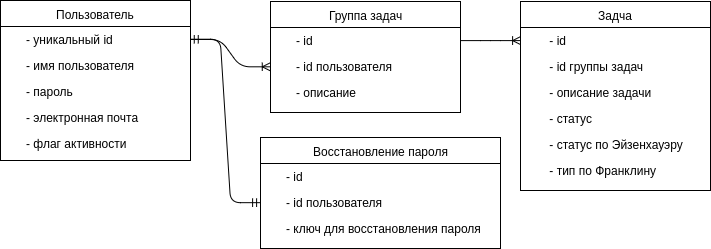
\includegraphics[scale=0.5]{images/entity-relation.png}  
  \caption{ Диаграмма сущность-связь для системы организации времени }
  \label{fig:domain:todist}
\end{figure}

Следом после построения диаграммы "сущность-связь", можно построить базы данных MySQL, определив типы полей.

\begin{figure}[ht]
\centering
  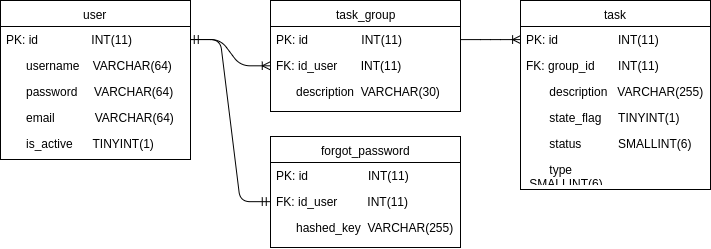
\includegraphics[scale=0.5]{images/mysql_schema.png}  
  \caption{ Схема базы даннных для системы организации времени }
  \label{fig:domain:todist}
\end{figure}